\begin{frame}
  \frametitle{Antisthenis}
  \framesubtitle{Dynamically scheduled incremental computation}

  Materializablility and cost inference are numerical operations:

  \begin{itemize}
  \item Input is mostly the same between runs: \textbf{incremental}.
  \item \textbf{Order of computation} highly affects the performance
    (eg absorbig elements, min).
  \item Self referrential computations may appear earlier than the
    absorbing element.
  \end{itemize}
\end{frame}


\begin{frame}
  \frametitle{Antisthenis: Expression graphs}
  \begin{columns}
    \begin{column}{0.5\textwidth}
      \begin{align*}
        A &= a + B + C + D  \\
        B &= C \times b \\
        C & = D + c \\
        D &= 0
      \end{align*}
    \end{column}
    \begin{column}{0.5\textwidth}
      \begin{center}
        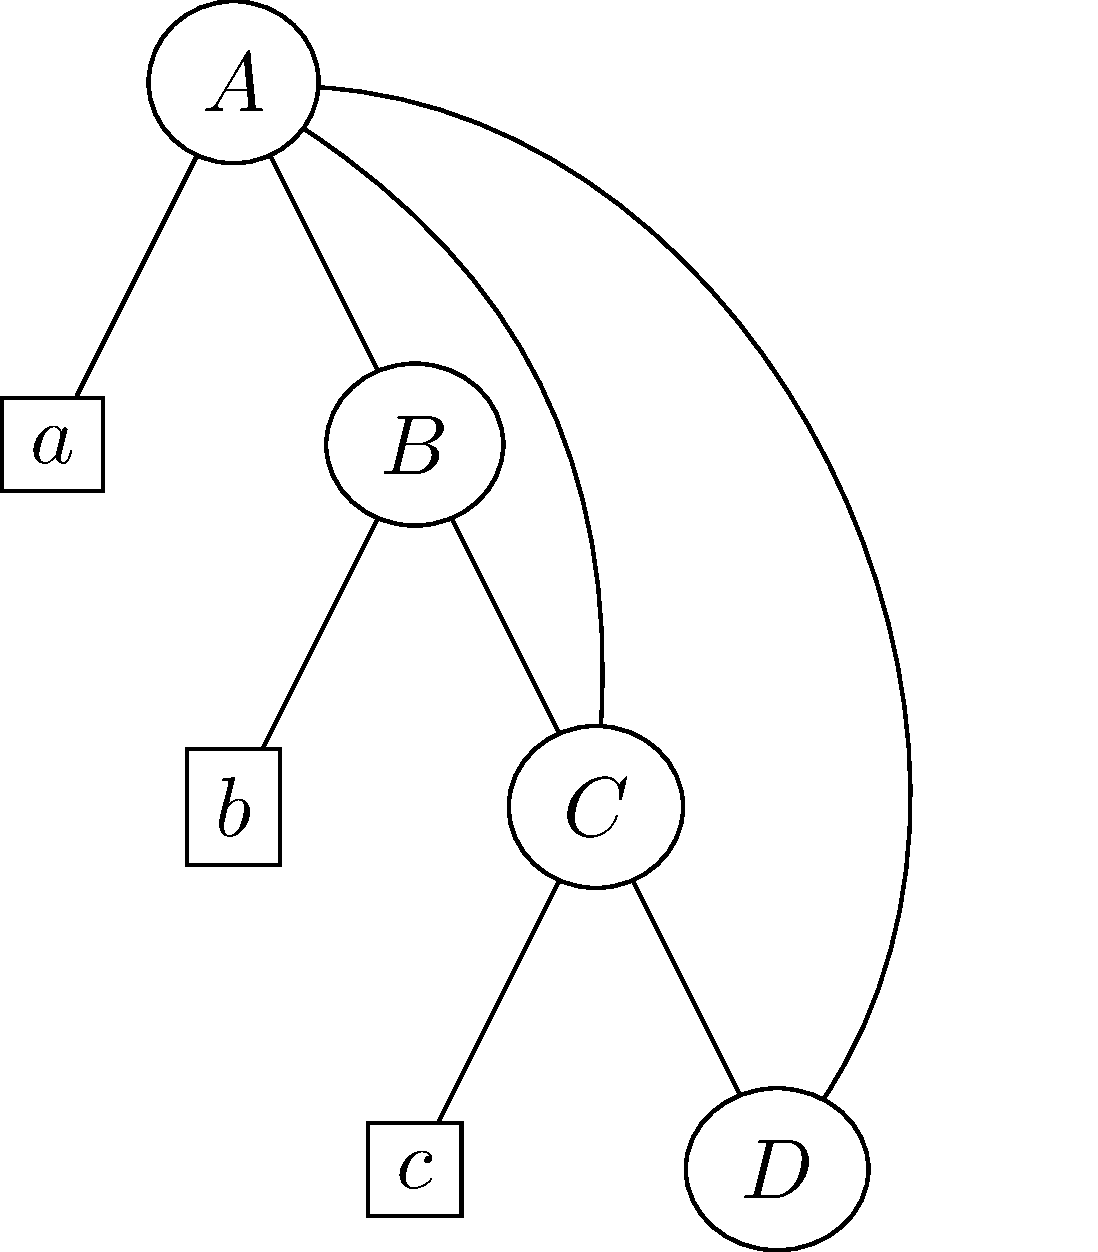
\includegraphics[height=.6\textheight]{../imgs/example_antisthenis_dag.pdf}
      \end{center}
    \end{column}
  \end{columns}
\end{frame}


\begin{frame}
  \frametitle{Antisthenis: Absorbing element}
  \begin{align*}
    A &= {\color{red}B} \times {\color{gray}C} \times D \\
    {\color{red}B} &= {\color{red}\sum_i{i}} \\
    {\color{gray}C} &= {\color{gray}10 - 10} \\
    D &= \sum_i{i}
  \end{align*}
\end{frame}


\begin{frame}{Antisthenis: Early stopping -- recursive expressions}
  {While expressions may be self-referential, we can
    sometimes still evaluate them.}
  \begin{align*}
    A &= min({\color{red}B}, C, {\color{blue}D}) \\
    {\color{red}B} &= b_1 + b_2 \cdot {\color{blue}D} \\
    C &= c_1 + {\color{gray}c_2 \cdot A} \\
    {\color{blue}D} &= d_1 + d_2 \cdot {\color{red}B} \\
  \end{align*}
  \hrule
  \begin{align*}
    b_1 &= b_2 = d_1 = d_2 = 1 \\
    c_1 &= 3 \\
    c_2 &= 0
  \end{align*}
\end{frame}

\newcommand{\wlor}{\mathop{\bigvee}\displaylimits}
\newcommand{\wland}{\mathop{\bigwedge}\displaylimits}
\begin{frame}{Kinds of operations: Materializability}
  \[
    matable(n) := \wlor_{depset \in depsets(n)}\wland_{dep \in depset} mat(dep) \lor matable(dep)
  \]
  \uncover<2>{
    \begin{itemize}
    \item Recursive -- normally we would maintain a visited set.
    \item Incremental evaluation is inhibited.
    \item Bot \(\land\) and \(\lor\) have absorbing elements.
    \end{itemize}}
\end{frame}

\begin{frame}{Kinds of operations: Estimated cost}
    \[
  \scalebox{0.7}{
    \(cost(n) := \min\limits_{depset \in depsets(n)}\left[cost_{op}(operator(depset)) + \sum_{dep \in depset}\neg mat(n) \cdot cost(dep)\right]\)
    }
    \]
  \uncover<2>{
    \begin{itemize}
    \item Recursive -- Incremental evaluation is inhibited.
    \item \(\min\) can be exploited for early stopping
    \end{itemize}}
\end{frame}
